\chapter{Grundlagen}\label{kap:grundlagen}
\section{Softcore-Prozessoren}\label{kap:softcoreprozessoren}

Ein SoftCore (engl. „Software-Kern“) ist ein Prozessor, Mikrocontroller oder ein Signalprozessor, welcher als virtuelle Einheit in einem \ac{fpga} oder \ac{asic} integriert wird.
Dies bietet die Möglichkeit einem digitalen Schaltungsdesign jeden beliebigen Prozessor hinzuzufügen.\\
Umgesetzt wird dieser Vorgang im \ac{fpga} durch reine Anwenderlogik,
welche dementsprechend konfiguriert werden muss.\\
Das typische Anwendungsgebiet eines SoftCores ist die Lösung von komplizierten Aufgaben, mit denen klassische „State Machines“ überfordert sind oder die Effektivität
 nicht mehr gegeben ist. Somit werden SoftCores oftmals nachträglich in bestehende Designs eingefügt, wenn deren Umfang sich extrem vergrößert hat.\cite{softcore}\\

\subsection{Vergleich SoftCores und HardCores}\label{kap:vergleich}

Vergleicht man den SoftCore- mit dem HardCore-Prozessor, lassen sich folgende Aussagen treffen:

Vorteile:
\begin{itemize}
   \item Flexible Anwendung: Das \ac{fpga} kann bei Bedarf mit einem SoftCore versehen werden, jedoch wird nicht von vorneherein Platz für einen HardCore verschwendet, welcher
    dann letztendlich ungenutzt bleibt. Daraus ergeben sich deutliche Vorteile im Hinblick auf die Kosten.
    \item Konfigurierbarkeit: Beim SoftCore deutlich flexibler, da hier unter anderem die Größe der Datenpfade und die Anzahl der Zusatzmodule variiert werden kann.
 \end{itemize}


Nachteile:
\begin{itemize}
  \item SoftCores haben auf Grund ihrer Flexibilität einen deutlichen Geschwindigkeitsnachteil
\end{itemize}

\subsection{Typen}\label{kap:typen}
Es gibt eine große Anzahl verschiedener SoftCores. Diese unterscheiden sich aber maßgeblich in der Größe der Datenpfade.
Somit wird unterschieden zwischen 8-,16- und 32-Bit Systemen.\cite{softcore}\\

\textbf{8-Bit SoftCores}\\
\begin{table}[H]
\centering
\begin{tabular}{|l|c|r|}
  \hline
  \textbf{Name} & \textbf{Quellcode} & \textbf{Hersteller}\\
  \hline
  LatticeMico8 & Verilog und VHDL & Lattice\\
  \hline
  PicoBlaze & VHDL & Xilinx\\
  \hline
  Proteus & VHDL & LogicSolutions\\
  \hline
\end{tabular}
  \caption{8-Bit SoftCores nach ~\cite{softcore}}
 \label{tab:8bitsysteme}
  \end{table}

  \textbf{16-Bit SoftCores}\\
  \begin{table}[H]
  \centering
  \begin{tabular}{|l|c|r|}
    \hline
  \textbf{Name} & \textbf{Quellcode} & \textbf{Hersteller}\\
    \hline
    NEO430 & VHDL & neo430@GitHub\\
    \hline
    OpenMSP430 & Verilog & OpenCores\\
    \hline
    TG68 & VHDL & OpenCores\\
    \hline
  \end{tabular}
    \caption{16-Bit SoftCores nach ~\cite{softcore}}
   \label{tab:16bitsysteme}
    \end{table}

    \textbf{32-Bit SoftCores}\\
    \begin{table}[H]
    \centering
    \begin{tabular}{|l|c|r|}
      \hline
    \textbf{Name} & \textbf{Quellcode} & \textbf{Hersteller}\\
      \hline
      LEON & VHDL & Gaisler Research\\
      \hline
      MicroBlaze & Nein & Xilinx\\
      \hline
      OpenRISC & Verilog & OpenCores\\
      \hline
      NIOS II & Nein & Altera\\
      \hline
    \end{tabular}
      \caption{8-Bit SoftCores nach ~\cite{softcore}}
     \label{tab:8bitsysteme}
      \end{table}








\section{Memory Management Unit}\label{kap:mmu}

Bei der \ac{mmu} handelt es sich um einen Hilfsbaustein des Betriebssystems, welcher die Speicherverwaltung des Arbeitsspeichers beschleunigt. Umgesetzt wird diese Verwaltung mit
Hilfe eines Verfahren, welches virtuelle Adressen auf physikalische Adressen abbildet. Der gesamte Speicher wird in einzelne Speicherbereiche unterteilt und die
\ac{mmu} überwacht die Einhaltung dieser Bereiche und unterbricht gegebenenfalls Instruktionen, die auf einen verbotenen
Bereich zugreifen wollen.\cite{itwissen}\\

\begin{figure}[H]
\centering
\includegraphics[width=0.8\textwidth]{Hauptteil/mmu.eps}
\caption{Blockschaltbild einer MMU}\label{fig:mmu}
\end{figure}


 \section{Peripherie}\label{kap:peripherie}
 Ein Peripheriegerät kann einer Hardware hinzugefügt werden, um die Fähigkeiten zu erweitern. Diese Geräte sind optional und dienen zur Ein- und Ausgabe von Daten.

\subsection{UART}\label{kap:uart}

Um mit Peripheriegeräten zu kommunizieren, kann \ac{uart} als serielle Schnittstelle genutzt.
Bei dieser Art der Kommunikation werden serielle Daten zwischen dem Board (\emph{Master})
und dem Empfänger (\emph{Slave}) ausgetauscht. \\
Dabei spielen die TxD und die RxD-Datenleitungen
eine wichtige Rolle, da der Datenaustausch über diese Leitungen realisiert wird.\\
Im Gegensatz, zum Beispiel, zu einer \ac{spi}-Schnittstelle, wird kein Clock-Signal
übertragen um Daten zu validieren. Des Weiteren wird die Verbindung mit einer definierten
Geschwindigkeit realisiert, der sogenannten \emph{Baudrate}. \cite{uartpdf} \\
Die Baudrate bezeichnet dabei die Anzahl der Bits, welche pro Sekunde übertragen werden.
\ac{uart} konvertiert die Bytes in serielle Bits, überträgt diese über eine einzelne Leitung
und liest die zugehörigen Start- und Stop-Bits aus.\\
Das sogenannte \emph{Character}(Zeichen) besteht aus einer konfigurierbaren Anzahl an Datenbits (in den meisten
Fällen 7 oder 8), aus einem \emph{low-level} Start-Bit , einem optionalen Parity-Bit und einem
oder mehreren logischen \emph{high-level} Stop-Bits.\\
Das Start-Bit teilt dem Receiver mit, dass ein neues \emph{Character} empfangen wird.
Die nächsten Bits, je nachdem wie viele Daten-Bits vorher konfiguriert wurden , stellen
dann den Inhalt des \emph{Character} dar. Darauf folgt das optionale Parity-Bit,
welches anzeigt, ob die Anzahl der mit '\emph{1}' belegten Daten-Bits gerade oder
ungerade ist. Am Ende der Folge stehen dann entweder ein oder zwei  \emph{high-level } Stop-Bits,
welche dem Receiver eindeutig signalisieren, dass die Übertragung vollständig ist. Dadurch,
dass das Start-Bit \emph{high-level} (1) und das Stop-Bit \emph{low-level} (0) ist,
ist immer eine klare Abgrenzung zwischen dem derzeitigen und dem folgenden \emph{Character} möglich.\\

Die Datenübertragung lässt sich nach~\ref{fig:uart} darstellen.\\

\begin{figure}[h!]
\centering
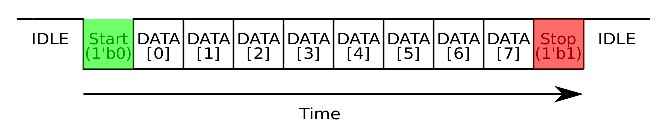
\includegraphics[width=0.8\textwidth]{Hauptteil/uart.eps}
\caption{Datenübertragung per \ac{uart}(8n1) }
\label{fig:uart}
\end{figure}


\subsection{Interrupt}\label{kap:interrupt}
Neben der \ac{cpu} und dem Datenspeicher haben die meisten Computersysteme Peripherie. Es handelt sich dabei um verbaute oder um an Schnittstellen angeschlossene Geräte.
Damit die \ac{cpu} die Nachricht erhält, dass Daten an solch einer Schnittstelle beziehungsweise Verbindung anliegen, muss es eine Möglichkeit geben den Prozessor zu
unterbrechen. Hier gibt es die Art des sogenannten Polling, bei dem der Prozessor alle vorhandenen Eingabegeräte zyklisch abfragt. Ein effektiveres Verfahren ist die
Unterbrechungsanforderung (Interrupt), welche eintritt, wenn Daten anliegen. \\
Sobald ein Gerät Daten zur Weiterverarbeitung besitzt, wird ein \ac{irq} auf der dafür vorgesehenen Interrupt-Leitung gesendet. Daraufhin unterbricht der Prozessor
seine Arbeit und verarbeitet die Daten des Gerätes.\cite{irq}\\

\begin{figure}[H]
\centering
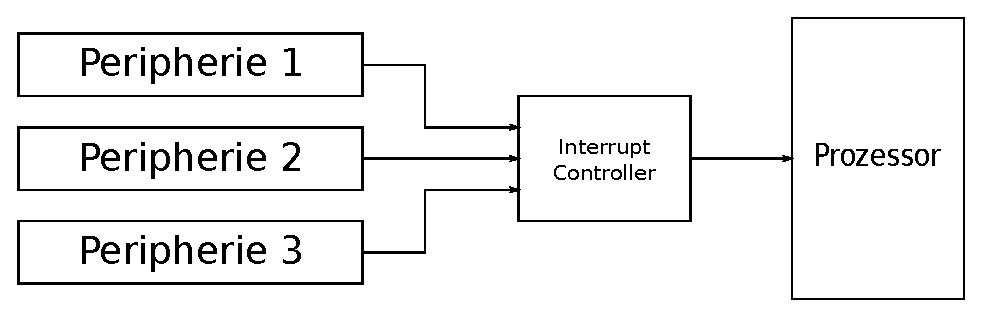
\includegraphics[width=0.8\textwidth]{Hauptteil/irq.eps}
\caption{Interrupt-Controller}\label{fig:irq}
\end{figure}

\subsection{Timer}\label{kap:timer}

Ein weiterer essenzieller Teil zur Ausführung eines Betriebssystems, wie zum Beispiel Linux, ist der Timer. Dieser hilft dem Betriebssystem dabei, das so genannte Scheduling
durchzuführen. Hierbei wird mit Hilfe von \emph{Timer}-gesteuerten Interrupts dafür gesorgt, dass Nutzerprogramme, welche sich in der Ausführung befinden, unterbrochen werden und
in den Betriebssystem-Modus geschaltet wird. Nun kann das Betriebssystem die anstehenden Prozesse neu planen.\\


\section{Compiler}\label{kap:compiler}

Der Compiler ist ein Werkzeug, welches einen Quelltext, der in einer höheren Programmiersprache (C++, C, Java) geschrieben wurde, in Maschinenbefehle umsetzt. Damit der Prozessor diese Instruktionen ausführen kann, werden die lesbaren Programmierbefehle übersetzt. Nach dem so genannten kompilieren steht das Programm zur Ausführung bereit.
Die Aufgaben des Compilers bestehen grundsätzlich aus drei Schritten:\cite{compiler}
\begin{enumerate}
  \item Lexikalische Analyse:
  	Der Compiler zerlegt die Wörter und Zeichen des Quelltextes in verschiedene Klassen. Dabei werden überflüssige oder fehlende Zeichen als Fehler erkannt und vom Compiler, je nach
  schwere des Verstoßes, als Warning oder Error ausgegeben.
  \item Parsing:
  	Es folgt die Prüfung des Codes auf syntaktische Korrektheit.
  \item Semantische Analyse: Der Quelltext wird auf Sinnhaftigkeit geprüft. Zum Beispiel ob Befehle wirklich die korrekten Parameter haben.
\end{enumerate}

Im Vergleich zum Interpreter gibt es folgende Vor- und Nachteile.

Vorteile:
\begin{itemize}
  \item effiziente Übersetzung in ausführbaren Code
  \item Optimierung des generierten Codes
\end{itemize}

Nachteile:
\begin{itemize}
  \item Kompilieren benötigt Zeit und Ressourcen
  \item Neu-Kompilierung nach Quelltextänderung
  \item Jede Programmiersprache benötigt einen eigenen Compiler
\end{itemize}

\begin{figure}[H]
\centering
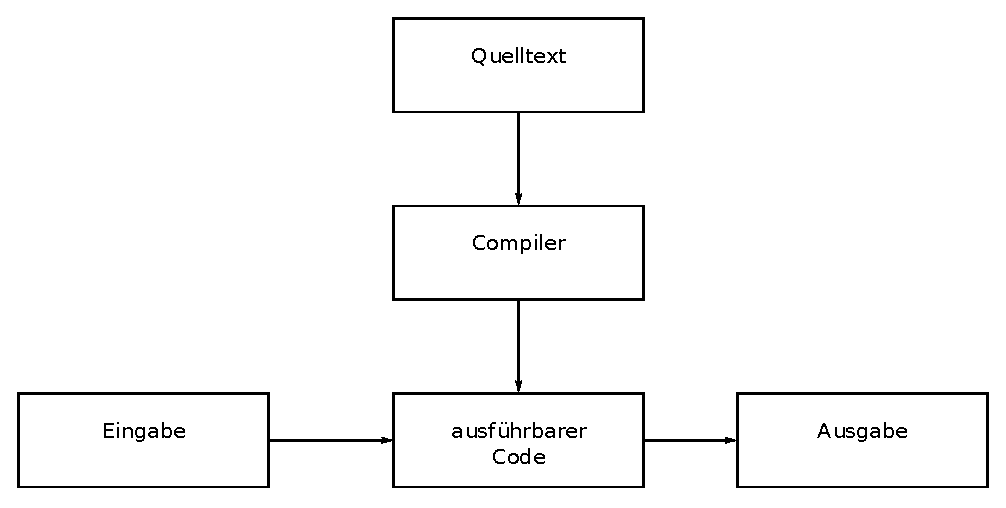
\includegraphics[width=0.8\textwidth]{Hauptteil/Compiler.eps}
\caption{Funktionsweise des Compilers}\label{fig:compiler}
\end{figure}

\subsection{Compiler-Modi}\label{kap:compilermode}
\begin{itemize}
  \item Non-OS mode: Programme ohne Zugriff auf Ein- bzw. Ausgabegeräte. Programme, welche in diesem Modus ausgeführt werden, haben keine periphere Unterstützung
        Der Bare-Metal-Mode wird meistens genutzt, um \ac{isa}- und Cache-Regressionstests durchzuführen. Hierbei entscheidet der Rückgabewert des Programmes über Erfolg beziehungsweise Misserfolg
        des Tests. \emph{0} bedeutet Erfolg, Zahlen ungleich \emph{0} geben den jeweiligen Fehlercode an. Bare-Metal-kompilierte Programm laufen auf einem \ac{fpga} und in einer Simulation
        im Hintergrund. \\
        Um nun mit einem Bare-Metal-Programm eine Ausgabe zu erzeugen, müssen Bibliothkenen verwendet werden, welche die Art und Weise der Ausgabe beinhalten.\\

        \begin{figure}[H]
        \centering
        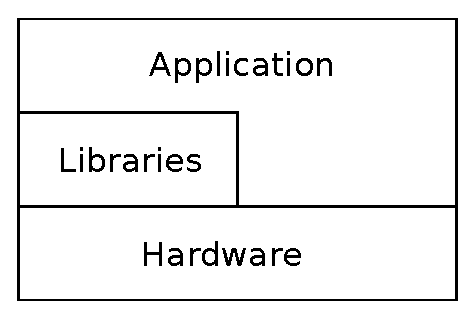
\includegraphics[width=0.4\textwidth]{Hauptteil/baremetal.eps}
        \caption{Grafische Darstellung der Non-OS-Architektur}\label{fig:baremetal}
        \end{figure}

  \item Linux mode: Benutzerprogramme mit Linux-Unterstützung. Mit Hilfe dieser Programme lassen sich Verhaltssimulationen auf dem \ac{fpga}-Board durchführen. Diese Programme
  erhalten Multi-Thread und Peripherie-Unterstützung vom Linux-Kernel\cite{lowrisc}\\

  \begin{figure}[H]
  \centering
  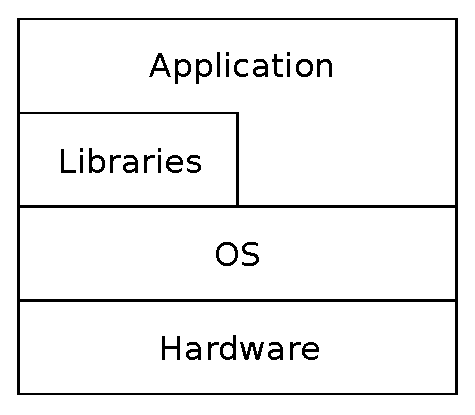
\includegraphics[width=0.4\textwidth]{Hauptteil/linuxmode.eps}
  \caption{Grafische Darstellung der Linux-Architektur}\label{fig:linuxmode}
  \end{figure}
\end{itemize}




\section{Linux}\label{kap:linux}


Das verwendete System Linux wurde als freies Betriebssystem von Linus Benedict Torvald entwickelt.
Es basiert auf dem Unix-Modell, jedoch schrieb Torvald den sogenannten Kernel neu. Seit dem gilt
Linux als Open-Source-Projekt und Entwickler versuchen stetig das System zu verbessern.\cite{linux}\\
Die wohl wichtigste Eigenschaft die Linux bzw. Unix für den Einsatz beliebt machen ist die Portabilität,
da es weitestgehend rechnerunabhängig läuft. Weitere Eigenschaften die das Betriebssystem zu einem der
 weitverbreitetsten Systeme überhaupt gemacht haben, sind:\\\cite{linux}\\
\begin{itemize}
\item  \textbf{Multi-Tasking} Das parallele Nutzen verschiedener Programme erlaubt jedem Benutzer
        gleichzeitige Aktionen durchzuführen, ohne auf den Abschluss der letzten Tätigkeit zu warten.
\item  \textbf{Time-Sharing} Das Priorisieren von einzelnen Prozessen erlaubt es, dass mehrere
        Prozesse gleichzeitig ablaufen, indem abwechselnd Platz im Hauptspeicher beziehungsweise in der \ac{cpu}
        zugewiesen wird.
\item \textbf{Sprachenvielfalt} Neben der Sprache C stellt Linux/Unix viele Programmiersprachen
      wie C++, Java, Python und viele mehr zur Verfügung. Dadurch, dass es sich um ein Open-Source-Projekt handelt,
      wird diese Bibliothek, je nach System, ständig erweitert.
\item \textbf{Grafische Benutzeroberfläche} Linuxrechner, im speziellen die Anwendungen, nutzen in
      den meisten Fällen \ac{gnome} oder \ac{kde} als grafische Oberfläche. Durch die weitverbreitete Nutzung
      dieser Oberflächen wurden diese kontinuierlich weiterentwickelt und bieten so eine hohe Vielfalt an
      Anpassungsmöglichkeiten.
\item \textbf{Netzwerk} Für die Kommunikation zwischen Server und Client hat sich das Betriebssystem bewährt,
      da es über ein umfangreiches Paket an Software verfügt. Neben den Standardprotokollen \ac{tcpip} (IPv6 wird
      ebenfalls unterstützt), werden weitere Formate verwendet, wie zum Beispiel \ac{uucp}, welches eine simple Form
      der Kommunikation zwischen Linux/Unix-Rechnern darstellt.
\end{itemize}

Grundsätzliche bestehen Betriebssysteme wie Linux/Unix aus drei Hauptkomponenten.
Der \textbf{Kern} (engl. \emph{Kernel}) bildet die grundlegenden Funktionen, wie
zum Beispiel die Organisation und Verwaltung von Speicher, der Prozesse, sowie
Ein- und Ausgänge und sämtliche Kommunikationsaufgaben.\\
Das \textbf{Dateisystem} (engl. \emph{File System}) ermöglicht das Speichern von Dateien
und errichtet einen Dateibaum und ist somit für die Datenorganisation zuständig.\\
Die dritte Komponente stellt der \textbf{Befehlsübersetzer} dar (engl. \emph{shell}),
welcher anhand einer Befehlssprache die Kommunikation ermöglicht und dem Benutzer erlaubt
mit sämtlichen Peripheriegeräten zu interagieren, ohne dass die im Hintergrund laufenden
Prozesse berücksichtigt werden müssen. \cite{ubuntu}\\

Grafisch lässt sich der Aufbau wie folgt darstellen:\\

\begin{figure}[H]
\centering
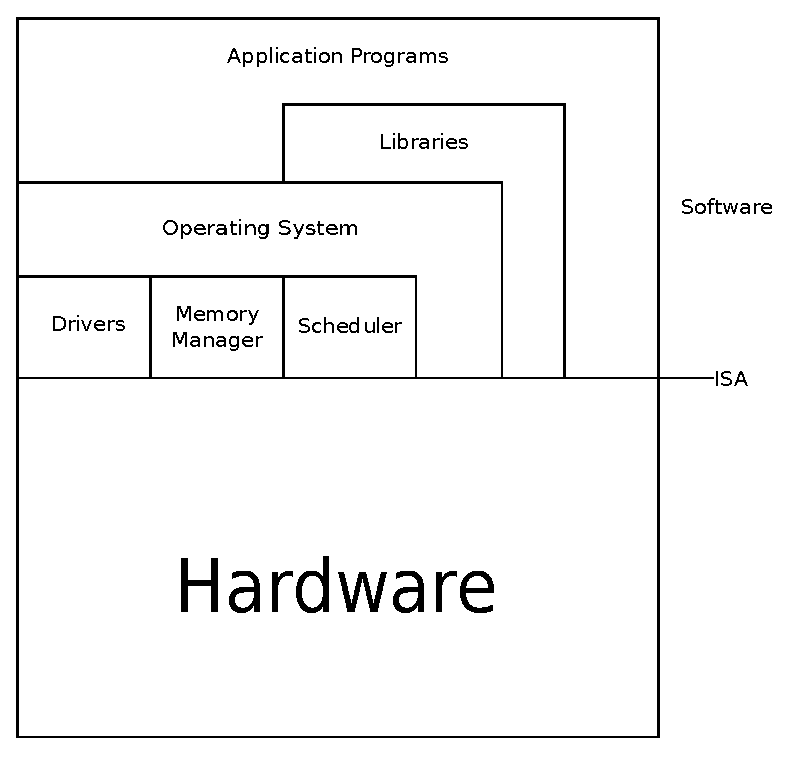
\includegraphics[width=0.55\textwidth]{Hauptteil/csa.eps}
\caption{Computer System Architektur nach \cite{virtualmachines}}
\label{fig:mbs}
\end{figure}

Um nun mit den verschiedenen Geräten über eine Vielzahl von Schnittstellen kommunizieren
zu können, benötigt jedes Gerät einen eigenen Treiber. Dieser Treiber ist im Betriebssystem
als \emph{„Wissen“} hinterlegt und beinhaltet Information über das Gerät und dessen
Zugriffsmöglichkeiten und wird im folgenden Unterkapitel näher erklärt. \cite{treiber}\\
Der Anwender hat nun die Möglichkeit über die Treiber auf die Schnittstellen zuzugreifen, in dem diese vom
Treiber gesteuert werden.

\subsection{Treiber}\label{kap:treiber}

Der Treiber gilt als \emph{„Lexikon“} der jeweiligen Geräte für das Betriebssystem.
Diese Aufgabe ist enorm wichtig für ein funktionierendes System, sodass der Stellenwert
eines Treibers sehr hoch ist. Einfach erklärt, besteht ein Treiber aus einer Reihe von
Funktionen, die den Zugriff auf das Gerät steuern und so eine Kommunikation ermöglichen.
So muss für jedes Gerät ein eigener Treiber implementiert werden, der die offene
Schnittstelle im Betriebssystemkern füllt. \\
Dabei sind zwei Begrifflichkeiten wichtig, in die der Speicherbereich aufgeteilt wird:
\begin{itemize}
\item \textbf{Kernelspace} : Diese Bereich wird ausschließlich vom Kernel benutzt
\item \textbf{Userspace} : Dieser Speicher wird von Applikationen genutzt und kann nicht,
                          oder in Ausnahmfällen, nur eingeschränkt vom Kernel genutzt werden
\end{itemize}

Die Treiber werden grundsätzlich mit in den Kernel kompiliert oder sind als Modul dynamisch
angelegt, um zum Kernel, während der Laufzeit, hinzugefügt zu werden. \cite{treiberbib}\\

Bei der Implementierung von Gerätetreibern wird zwischen drei Gerätetypen unterschieden (\cite{treiberbib}):\\
\begin{enumerate}
\item \textbf{Character-Devices} Auf diese Geräte kann wie auf einen Stream von Bytes zugegriffen werden, indem
      \ac{posix}-Funktionen genutzt werden, wie beispielsweise \emph{open()},\emph{write()},\emph{read()} oder \emph{close()}.
      Für die Nutzung wird für jedes Gerät eine \emph{Gerätedatei} (vgl. \emph{device nodes}) angelegt.
\item \textbf{Block Devices} Im Gegensatz zu den \emph{Character-Devices}, wird auf die \emph{Block-Devices} immer per Random Access zugegriffen.
      Die Daten werden blockweise gelesen. Diese \emph{Block-Devices} können ein Dateisystem aufnehmen und gemountet werden.
\item \textbf{Netzwerkschnittstellen} Netzwerkgeräte erhalten keine Gerätedatei, sondern sind in einer globalen Liste hinterlegt.
      Der Datenaustausch findet immer asynchron statt, sodass die Netzwerkkarte jederzeit bereit sein muss Daten zu empfangen.
\end{enumerate}


\subsubsection{Device Tree}\label{kap:devicetree}


Der \emph{Device-Tree} beinhaltet
Informationen, welche dem Kernel bei dem Bootvorgang helfen. Da das System angeschlossene Geräte nicht automatisch erkennen
und die dazu passenden Treiber laden kann, geschieht das in dieser \emph{.dts}-Datei. Durch das Kompilieren wird daraus
der sogennante \emph{Device} \emph{Tree} \emph{Blob}. Dieser wird zusammen mit dem Kernel vom Bootloader geladen und im
Hauptspeicher abgelegt. Im Anschluss daran wird daraus eine Baumstruktur. In dieser sind die Geräte als Knoten angelegt
und es werden Informationen zu den dazugehörigen Treiber hinterlegt, welche dem Betriebssystem zur Verfügung gestellt werden.
Die Verbindung zwischen Device-Tree und dem Treiber wird über eine
eindeutige Identifikation per \emph{Compatible} festgelegt.


\subsection{Buildroot}\label{kap:buildroot}

\emph{Buildroot} ist ein Tool, welches das Erstellen eines kompletten Linux-Systems per
\emph{Cross-Compiling} für eingebettete Systeme vereinfacht und automatisiert.  Neben dem
\emph{cross-compiled} Toolchain können ebenfalls das \emph{Root}-Dateisystem, ein \emph{Linux-Kernel-Image}
und ein \emph{Bootloader} für das Zielsystem erstellt werden.  In einem Konfigurationsprogramm lassen sich vor der
Erstellung sämtliche Optionen und Erweiterungen ab- beziehungsweise anwählen. \\
Das Tool wird größtenteils dafür genutzt, um die Systeme für andere Prozessoren, außer die klassischen x86-Prozessoren,
zu erstellen, wie zum Beispiel \ac{arm}-Prozessoren.\cite{buildroot}\\

\textbf{Toolchain}\\

Bei der \emph{Toolchain} handelt es sich um eine Reihe von Tools zum Erstellen und Debuggen von Code für eine Zielarchitektur. Des Weiteren beinhaltet sie einen Compiler, einen Linker,
 sowie verschiedene Bibliotheken.\\
 Die Toolchain ist essenziell, um die drei weiteren Elemente eines eingebetteten Systems zu generieren: den Bootloader, den Kernel und das Root-Dateisystem. \\
 Hierbei wird im wesentlichen zwischen zwei \emph{Toolchain}-Arten differenziert:
 \begin{enumerate}
   \item Die interne Toolchain: Die \emph{Toolchain} wird aus einer Quelle heraus vom \emph{Buildroot} generiert
   \item die externe Toolchain: Es wird eine bereits vorhandene \emph{Toolchain} verwendet
 \end{enumerate}

Das generieren einer eigenen \emph{Toolchain} benötigt entsprechend mehr Zeit und verlängert den ganzen Kompiliervorgang, bietet jedoch deutlich mehr Konfigurationsmöglichkeiten
im Vergleich zu bereits vorhandenen \emph{Toolchains}.\\

\textbf{Kernel}\\

Der \emph{Kernel}, welcher bereits in Kapitel~\ref{kap:linux} beschrieben wurde, kann ebenfalls durch \emph{Buildroot} konfiguriert und erzeugt werden.\\
Dieser steuert alle Prozessor-und Speicherzugriffe, unterhält die wichtigsten Treiber und freift direkt auf die Hardware zu. Dadurch, dass er die unterste Schicht des Systems beschreibt,
ist er die Basis in der Kommunikation zwischen Hard- und Software.\\
Zu seinen Aufgaben gehören neben der parallelen Verarbeitung verschiedener Aufgaben, auch die Einhaltung zeitkritischer Grenzen, sowie die Offenheit für unterschiedlichste Anwendungen
und Erweiterungen. Im Falle des Linux-Systems gilt der Kernel als Vermittler im System, so ist die grafische Oberfläche komplett unabhängig vom Linux-Kernel.\cite{datacenter}\\

\textbf{Root-Dateisystem}\\

Der Kernel enthält keine Programme oder Dämonen, die das System an sich nutzbar machen. Hierfür ist das \emph{Root-Dateisystem} zuständig.\\
Wichtige Inhalte sind:
\begin{itemize}
  \item init-Dämon: Startet Dämonen, Systemeinstellungen sowie Login-Programmen
  \item System-Konfiguration
  \item Device-Nodes
  \item Bibliotheken und Kernel-Module
\end{itemize}

Für die Zusammenstellung dieses Dateisystem kann \emph{Buildroot} verwendet werden, wodurch \emph{BusyBox} sowie weitere Programmpakete integriert werden.\cite{elektronikpraxis}\\

\textbf{Bootloader}\\

Der Bootloader, auch Boot Manager genannt, ist ein Programm, dessen Aufgabe es ist, das Betriebssystem in den Arbeitsspeicher zu laden. In diesem Fall ist er dafür verantwortlich,
den Kernel mit den gewünschten Parametern zu laden und den Speicher zu initialisieren, bevor der eigentliche Boot-Prozess startet.\cite{searchdatacenter}\\

\textbf{BusyBox}\\

BusyBox kombiniert winzige Versionen vieler gängiger UNIX-Dienstprogramme in einer einzigen kleinen ausführbaren Datei.
Es bietet Ersatz für die meisten Dienstprogramme, die normalerweise in GNU fileutils, Shellutils zu finden sind.
Die Dienstprogramme in BusyBox haben im Allgemeinen weniger Optionen als ihre voll ausgestatteten GNU-Gegenstücke, welche jedoch die erwartete Funktionalität bieten und vom Verhalten sehr ähnlich sind.
Ebenfalls bietet die BusyBox eine ziemlich vollständige Umgebung für eingebettete Systeme.\\
BusyBox wurde größenoptimiert und für begrenzte Ressourcen geschrieben.
Es ist auch extrem modular, so dass Befehle (oder Funktionen) zur Kompilierzeit ein- und ausgeschlossen werden können.
Dies erleichtert die schnelle Anpassung der eingebetteten Systeme.\cite{busybox}\\


\chapter{Soft Cores}\label{kap:softcores}
\section{MicroBlaze basierte Systeme}\label{kap:microblaze}
Microblaze

Der MicroBlaze SoftCore von Xilinx ist eine 32-Bit RISC Harvard Architektur mit einem umfangreichen Befehlssatz und ist optimiert für eingebettete Anwendungen.
Neben dieser Flexibilität besitzt er drei unterschiedliche Voreinstellungen:

\begin{enumerate}
  \item Microcontroller: Geeignet für Baremetall-Code
        \begin{itemize}
          \item 32-Bit Prozessorkern (in der Regel ohne \ac{mmu})
          \item Externer Speichercontroller
          \item \ac{spi} Controller
          \item I2C-Controller
          \item \ac{uart}
          \item Interrupt-Controller
          \item  Timer
        \end{itemize}
  \item Echtzeitprozessor: Deterministische Echtzeitverarbeitung auf einem \ac{rtos}
    \begin{itemize}
      \item Alle Mikrocontroller Blöcke
      \item Instruktioncache
      \item \ac{mpu}
      \item Datencache
      \item DDR-Controller
      \end{itemize}
  \item Anwendungsprozessor: Embedded Linux-fähig
        \begin{itemize}
          \item Alle Echtzeit-Prozessor-Blöcke
          \item 32-Bit-Prozessorkern
          \item \ac{mmu}
          \item Ethernet-Controller
        \end{itemize}
\end{enumerate}

Ausgehend von diesen Presets lässt sich das Design mit Hilfe von spezifischen Prozessoroptionen anpassen.
 Diese Vielanzahl an Anpassungen sind per Drag \& Drop sehr einfach hinzuzufügen. Dazu zählen unter anderem \ac{uart}-,\ac{pwm}- und \ac{dma}-Bausteine, sowie serielle Schnittstellen.
 Dadurch wird sichergestellt, dass die spezifischen Anforderungen der Anwendung erfüllt werden.

Zusammengefasst besitzt der Microblaze folgende Schlüsselfähigkeiten:
\begin{itemize}
  \item 32 mal 32-Bit-\emph{General-Purpose}-Register
  \item 32-Bit-Befehlswort mit drei Operanden und zwei Adressierungsmodi
  \item 32-Bit-Adressbus, erweiterbar auf 64-Bit
  \item Optionale \ac{fpu}
  \item \ac{axi}4-Interface
  \item Verschiedene Zustandsmodi (Sleep, Hibernate, Suspend Mode/Instrctions)
  \item Unterstützt entweder \ac{plb}- oder \ac{axi}-Schnittstellen
  \item Big-Endian / Little-endian Unterstützung
  \item Optionale \ac{mmu}, sowie separate, konfigurierbare Daten- und Instruktionscaches
\end{itemize}


\subsection{Erstellen der Hardwarekonfiguration}\label{kap:microblazehardware}


\textbf{Erstellen eines Projekts}\\\\
Starten Sie Vivado und wählen Sie \emph{New Project} aus.
Hierbei wählt man \emph{RTL Project} als Projekttyp, wobei der Haken bei \emph{"Do not specify sources at this time"} gesetzt sein sollte.\\
Nun gilt es unter dem Tab \emph{Boards} das korrekte Board auszuwählen, in meinem Fall war es das Nexys4 DDR.
Anschließend klicken Sie auf \emph{Finish} und das Projekt wird erstellt.\\


\newpage
\textbf{Erstellen des Block Designs}\\\\
Im Flow Navigator  auf der linken Seite wählt man nun \emph{Create Block Design} aus und
 gibt diesem Design einen beliebigen Namen.
Es öffnet sich das Block Design, bei dem der Tab \emph{Board} zu wählen ist. Hier werden nun
alle passenden Bausteine für das Nexys4 DDR-Board angezeigt.\\\\

\begin{figure}[H]
\centering
\includegraphics[width=0.4\textwidth]{Hauptteil/schritt3.png}
\caption{IP Integrator Block Design Diagram}\label{fig:mbschritt3}
\end{figure}

\vspace{10mm}


\textbf{Hinzufügen der Bausteine}\\\\
Durch doppeltes Klicken auf die Bausteine werden zunächst die \emph{System Clock}, \emph{USB UART} und \emph{DDR2 SDRAM} hinzugefügt. Die folgenden Fenster werden jeweils mit OK bestätigt.
Im Design Diagram kann nun über das „+“-Symbol der Microblaze und der \emph{\ac{axi} Timer} eingefügt werden.\\

\newpage
\textbf{Konfiguration des Clocking Wizard}\\\\
Der \emph{Clocking Wizard} muss wie im folgenden Bild konfiguriert werden.\\

\vspace{10mm}

\begin{figure}[H]
\centering
\includegraphics[width=0.8\textwidth]{Hauptteil/Schritt5.png}
\caption{Einstellungen des Clocking Wizard}\label{fig:mbschritt5}
\end{figure}

\vspace{10mm}

Dabei wird eine zweite Output Clock auf 200MHz gesetzt, sowie der Reset Type auf „Active Low“.\\

\newpage

\textbf{Anpassung der bestehenden Verbindungen}\\

Die bestehende Verbindung zwischen der SysClock und dem MIG muss gelöscht werden und eine neue Verknüpfung zwischen dem Clocking Wizard und dem MIG erstellt werden.\\

\begin{figure}[H]
\centering
\includegraphics[width=0.8\textwidth]{Hauptteil/schritt6.png}
\caption{Neue Verbindung zwischen ClkWiz und MIG7}\label{fig:mbschritt6}
\end{figure}

\vspace{10mm}

\textbf{Block Automation}\\

Ab hier greift die \emph{Block Automation} ein, bei der die im nachfolgenden Bild angezeigten Einstellungen zu übernehmen sind.
Besonders wichtig ist hier die Auswahl des Interrupt Controller.

\begin{figure}[H]
\centering
\includegraphics[width=0.65\textwidth]{Hauptteil/schritt7.png}
\caption{Einstellungen der Block Automation}\label{fig:mbschritt7}
\end{figure}


Im Anschluss wird die \emph{Connection Automation} gestartet und alle Bausteine ausgewählt.
Durch die Schaltfläche \emph{Regenerate Layout} kann das Diagram neu angeordnet werden.\\

\textbf{Manuelle Verbindungen}\\

Der angelegte Interrupt Controller ist mit einem \emph{Concat} verbunden, auf dessen Eingänge manuell die Interruptleitungen des \ac{axi} Uartlite und des \ac{axi} Timers gelegt werden.
Die Verbindungen sind im folgenden Bild orange gekennzeichnet.\\\\

\begin{figure}[H]
\centering
\includegraphics[width=1\textwidth]{Hauptteil/Schritt8.png}
\caption{Manuell erzeugte Verbindungen der Interruptleitungen}\label{fig:mbschritt8}
\end{figure}

\newpage

\textbf{Microblaze Konfiguration}\\

Der sogenannte MicroBlaze Configuration Wizard ermöglicht es, bereits voreingestellte Konfigurationen zu wählen.

\begin{itemize}
  \item Minimum Area: Minimaler MicroBlaze Core, kein Cache und kein Debug
  \item Maximum Performance: Maximale Leistung, großer Cache und Debug
  \item Maximum Frequency: Maximale Frequenz, kein Cache und kein Debug mit wenigen Ausführungseinheiten
  \item Linux with \ac{mmu}: Hohe Leistung, Linux-optimiert,\ac{mmu} aktiviert, großer Cache und Debug
  \item Low-end Linux with \ac{mmu}: Für low-end-Systeme, \ac{mmu} aktiviert, kleiner Cache und Debug
  \item Typical: Kompromiss zwischen Leistung, Frequenz und Größe
  \item Frequency Optimized: Bestmögliche Frequenz, \ac{mmu} aktiviert
\end{itemize}

  Der Microblaze ist wie folgt durch einen Doppelklick zu konfigurieren.

\begin{figure}[H]
\centering
\includegraphics[width=0.65\textwidth]{Hauptteil/microkonf.png}
\caption{Konfiguration des MicroBlaze}\label{fig:mbschritt9}
\end{figure}
Die neuen Einstellungen werden durch das Klicken des OK-Buttons übernommen.\\

\textbf{Anpassung des AXI Uartlite-Bausteins}\\

Der AXI Uartlite-Baustein muss ebenfalls angepasst werden. Hierbei gilt es im Tab „IP Configuration“ die Baudrate auf 115200 anzupassen.
Diese Änderung ist mit OK zu bestätigen.\\

\begin{figure}[H]
\centering
\includegraphics[width=0.65\textwidth]{Hauptteil/Schritt10.png}
\caption{Änderung der Baudrate des AXI Uartlite}\label{fig:mbschritt10}
\end{figure}

\vspace{10mm}

\textbf{Erstellen des HDL Wrappers}\\

Durch das Klicken der rechten Maustaste auf das Design im Source-Tab wird nun der HDL Wrapper erstellt.\\

\textbf{Generierung des Bitfiles}\\

Im nächsten Schritt wird das Bitfile generiert. Dafür ist im Flow Manager der Button „Generate Bitstream“ vorgesehen.
 Die „Number of jobs“ erhöht dabei die Geschwindigkeit je nach Prozessor und verfügbaren Kernen.\\
 Im Anschluss wird über File -> Export -> Export Hardware das generierte Bitstream für die SDK, welche als nächstes gestartet wird, nutzbar gemacht.\\


\textbf{Device Tree}\\

Um den dazugehörigen Device Tree zu generieren, wird das Device-Tree
 Repository benötigt, welches aus dem Xilinx Github runtergeladen werden kann: \url{https://github.com/Xilinx/device-tree-xlnx.git}\\
Nach dem Entpacken wird der Ordner nun im \ac{sdk} als Repository eingebunden.
 Dies geschieht über die Schaltfläche „Xilinx Tools“ beziehungsweise Repositories.
  Hier kann nun der Pfad des Ordners nur für ein bestimmtes Projekt oder für alle Projekte hinterlegt werden.\\

\textbf{Erzeugen des Board Support Packages}\\

Das Erstellen des Device-Tree geschieht über „File“ und anschließend „New“, sowie den Button „Board Support Package“.
Dabei sollte nochmal die voreingestellten Parameter überprüft werden und als Board Support Package OS
\emph{devicetree} ausgewählt werden.

\begin{figure}[H]
\centering
\includegraphics[width=0.8\textwidth]{Hauptteil/Schritt14.png}
\caption{Erstellen eines Device-Tree als Board Support Package}\label{fig:mbschritt14}
\end{figure}

Das folgenden Fenster kann ohne Weiteres mit OK bestätigt werden.\\


\textbf{Zusammenführung der \emph{Device Tree Source}-Dateien}\\

Die entstandenen \emph{.dtsi} beziehungsweise \emph{.dts}-Dateien müssen zusammengeführt werden und in einer \emph{.dts}-Datei gespeichert werden.
Hierzu sind beide Dateien im Texteditor zu öffnen, um die \emph{.dts}
 in die \emph{.dtsi}-Datei zu kopieren.
 Die resultierende Datei wird, wie bereits erwähnt, als alleinstehende \emph{.dts}-Datei gespeichert, um später in das buildroot-Tool eingefügt zu werden.\\

 \begin{lstlisting}[caption={Artix7.dts-Datei},label={code:artixdts}]
 /dts-v1/;
 / {
  #address-cells = <1>;
  #size-cells = <1>;
  compatible = "xlnx,microblaze";
  model = "Xilinx MicroBlaze";
  chosen {
    bootargs = "console=ttyUL0,115200";
    linux,stdout-path = &axi_uartlite_0;
    stdout-path = &axi_uartlite_0;
  };
  aliases {
    serial0 = &axi_uartlite_0;
  };
  memory {
    device_type = "memory";
    reg = <0x80000000 0x8000000>;
  };
  cpus {
    #address-cells = <1>;
    #cpus = <1>;
    #size-cells = <0>;
    microblaze_0: cpu@0 {
  \end{lstlisting}


\textbf{Buildroot}\\

Das bereits genannte Buildroot kann unter \url{https://buildroot.org/download.html} heruntergeladen werden.
Das in dieser Arbeit verwendete Buildtool besitzt die Version 2018.02.\\
Neben dem Buildroot werden Linux Kernel \emph{defonfig}-Dateien benötigt, welche für das Nexys4 angepasst wurden und auf folgenden Github zur Verfügung stehen :

\url{https://github.com/HenW/microblaze/tree/master}

Die Dateien werden in das Verzeichnis \emph{/board/nexys/microblaze} kopiert, welche vorher neu angelegt werden müssen.
 Es ist wichtig zu beachten, dass die Basisadresse des Kernels als 0x80000000 gesetzt ist und gegebenenfalls angepasst werden muss.

Die im vorherigen Schritt erstellte \emph{.dts}-Datei muss ebenfalls in das erstellte Verzeichnis eingefügt werden.\\

Des weiteren muss die Buildroot defconfig-Datei „nexys\_microblaze\_defconfig“ im \emph{configs}-Ordner abgelegt werden.\\

\textbf{Einrichten der Konfigurationsdatei}\\

Nachdem das System, wie in der vorherigen Schritt beschrieben,
vorbereitet wurde, muss nun folgender Befehl mit Hilfe eines Terminals im Buildroot-Verzeichnis ausgeführt werden:\\

\begin{lstlisting}[caption={Generierung der \emph{defconf}-Datei},label={code:mbdefconf}]
  make nexys_microblaze_defconfig
 \end{lstlisting}


Dieser Befehl erzeugt eine sogenannte .config Datei für das zugehörige buildroot.\\

\textbf{Erzeugen des Kernels}\\

Um den Kernel und das passende Filesystem zu erstellen, wird der Befehl \emph{make} benötigt.\\

\begin{lstlisting}[caption={Erstellung des Kernels},label={code:mbkernel}]
  make
   \end{lstlisting}

Dieser Vorgang benötigt je nach Rechenleistung einige Minuten.
Nach erfolgreichem Abschluss des Vorgangs wird eine „simpleImage.artix7“-Datei erstellt,
welche zum booten des Linux auf dem Nexys4 DDR Artix7 \ac{fpga} Modul benötigt wird.

\subsection{Ausführen des Linux Images auf dem Artix7}\label{kap:mcausführenlinux}



Das Linux Image muss jetzt in einen Ordner kopiert werden, welcher im Anschluss über
die \ac{sdk} Shell leicht zu erreichen ist. Das \ac{fpga}-Board wird nun mit dem Rechner über \ac{usb} verbunden und eingeschaltet.
 Über das Xilinx \ac{sdk} kann nun eine Verbindung über den korrekten Port mit der entsprechenden Baudrate (115200)
 hergestellt werden.\\

\textbf{Starten der \ac{xmd}-Engine}\\

Um die Verbindung zu prüfen kann, nachdem das \ac{fpga}-Board programmiert wurde, ein Hello World Programm ausgeführt werden. Andernfalls kann direkt im SDK über Xilinx Tools, beziehungsweise  „Launch Shell“ ein Terminal geöffnet werden.\\

Mit dem Befehl:

\begin{lstlisting}[caption={Öffnen des \ac{xmd}},label={code:mbxmd}]
  XMD
   \end{lstlisting}


wird eine \ac{xmd} Engine gestartet.\\

Anschließend wird über\\
\begin{lstlisting}[caption={Herstellen der Verbindung zum \acl{mb}},label={code:mbtarget}]
connect mb mdm
   \end{lstlisting}

eine Verbindung zum \ac{mb} als \ac{mdm} hergestellt.

Nun gilt es das Kernel Image auf das \ac{fpga}-Modul zu laden.
Hierzu muss innerhalb des Shells in den korrekten Ordner navigiert werden.
Über die bestehende Verbindung kann nun mit Hilfe von
\begin{lstlisting}[caption={Download des Images},label={code:mbimage}]
  dow simpleImage.artix7
   \end{lstlisting}

das Image heruntergeladen werden.
\newpage
\section{lowRISC basierte Systeme}\label{kap:lowrisc}

\textbf{Installation der benötigten Tools}

Um die RISC-V Tools erstellen zu können, werden verschiedene Pakete benötigt, welche vorher zu installieren sind.
\begin{itemize}
  \item autoconf: Produziert Shell Skripte zur automatischen Konfiguration von Software
  \item automake: Tool zur Generierung von Makefile-Dateien
  \item autotools-dev: Erneuert die Infrastruktur für config-Dateien
  \item libmpfr-dev: Mehrfach genaue Arithmetikbibliothek – Entwicklungswerkzeuge
  \item libmps-dev: siehe libmpfr-dev
  \item libgmp-dev: siehe libmpfr-dev
  \item gawk: GNU-Projekt Implementierung der AWK Programmiersprache
  \item build-essentials: Benötigte Pakete zur Kompilierung eines Pakets
  \item bison: YACC-kompatibeler Parser-Generator
  \item flex: schneller lexikalischer-Analysator
  \item texinfo: hypertextfähiges Dokumentationssystem
  \item gperf: Hash-Funktionsgenerator
  \item libncurses5-dev: Ncurses-Bibliotheken für Entwickler
  \item libusb-1.0.-0: Programmbibliothek zum Schreiben und Lesen von USB-Geräten
  \item libboost-dev: Boost C++ Bibliotheken
  \item Git: Software zur Versionsverwaltung von Dateien
\end{itemize}


\begin{lstlisting}[caption={Installation der benötigten RISC-V-Tools},label={code:riscvtools}]
Sudo apt-get install autoconf automake autotools-dev curl \
Libmpc-dev libmpfr-dev libgmp-dev gawk build-essential bison \
Flex texinfo gperf libncurses5-dev libusb-1.0-0 libboost-dev \
Git
\end{lstlisting}


\textbf{Download des lowRISC-Git-Repository}\\

Hierbei ist es empfehlenswert, dass gesamte Repository zu klonen, statt einzelne Untermodule.\\

\begin{lstlisting}[caption={Download des Repositories},label={code:riscrepository}]
cd ~/lowRISC/DIR
#download des untether-v0.2-Branch
git clone -b untether-v0.2 -recursive https://github.com/lowrisc/lowrisc-chip.git
cd lowrisc-chip
\end{lstlisting}


\vspace{5mm}
\textbf{Setzen der RISCV-Variablen}\\

Um die passende Umgebung zu schaffen, müssen die Variablen gesetzt werden. Hierfür ist zu erst der \emph{TOP}-Pfad anzugeben:\\

\begin{lstlisting}[caption={Setzen der TOP-Variable},label={code:topvariable}]
export TOP=[Gesamter Pfad zu dem lowRISC-Verzeichnis]
\end{lstlisting}



Bevor nun das Setupskript \emph{lowrisc-chip/set\_riscv\_env.sh} ausgeführt wird, um die restlichen Variablen anzupassen, muss in diesem Skript das passende Board angegeben werden.
Im Falle des verwendeten Boards Nexys4DDR wie folgt:\\

\begin{lstlisting}[caption={Anpassung des Zielsystems},label={code:zielsystem}]
[...]
#choose the FPGA board (KC705 in default)
export FPGA_BOARD=nexys4
\end{lstlisting}


Ausgeführt wird die angepasste Datei im Terminal mit:\\

\begin{lstlisting}[caption={Umgebungsvariablen},label={code:umgebungsvariablen}]
source set_riscv_env.sh
\end{lstlisting}

Es gilt zu beachten, dass das Einrichten dieser Umgebung jeweils nur für das genutzte Terminal gilt. Wird ein neues beziehungsweise ein weiteres Terminal geöffnet, müssen vorherigen Schritte erneut ausgeführt werden.\\

\textbf{Bauen des RISC-V Cross-Kompilierung-Tools}\\

In dem Repository wurde ein Skript mitgeliefert, welches die meisten Tools für die Cross-Kompilierung und Spike vorbereitet.
Dazu gilt es in den \emph{\$TOP/riscv-tools}-Ordner zu navigieren und das Skript
auszuführen.\\

\begin{lstlisting}[caption={Ausführen des \emph{build}-Skripts},label={code:buildskript}]
./build.sh
\end{lstlisting}



Nach der erfolgreichen Kompilierung sollten der Cross-Compiler, sowie Spike zur Verfügung stehen. Geprüft werden kann dies mit:\\

\begin{lstlisting}[caption={Überprüfung der Erreichbarkeit des Compilers},label={code:elfgcc}]
which riscv64-unknown-elf-gcc
\end{lstlisting}


\vspace{5mm}
\textbf{Erstellen des Linux-Cross-Compilers}\\

Neben dem RISCV-Cross-Compiler, welcher für das System an sich benutzt wird, wird ebenfalls ein Cross-Compiler für Programme, welche unter Linux ausgeführt werden sollen, benötigt.

Hierfür werden lediglich die Variablen innerhalb der RISCV-Umgebung angepasst.\\

\begin{lstlisting}[caption={Anpassung der RISCV-Umgebung},label={code:riscvumgebung},extendedchars=false]
cd $TOP/riscv-tools/riscv-gnu-toolchain
#wenn der Ordner "build" bereits existiert, kann der nächste Schritt ignoriert werden
mkdir build
cd build
../configure –prefix=\$RISCV
make –j(Anzahl Prozessorkerne) linux
\end{lstlisting}

\newpage
Auch hier kann die Verfügbarkeit überprüft werden.\\

\begin{lstlisting}[caption={Überprüfung der Erreichbarkeit des Linux-Compilers},label={code:linuxgcc}]
which riscv64-unkown-linux-gnu-gcc
\end{lstlisting}

\vspace{5mm}

 \textbf{Kompilieren des Linux Kernel}\\

Für den Linux Kernel, welcher mit Hilfe von Spike simuliert oder auf dem FPGA-Board gebootet werden kann, muss ebenfalls die Umgebung angepasst werden.

Es werden verschiedene Dateien benötigt, die unter den folgenden Verlinkungen heruntergeladen werden können.\\

\begin{lstlisting}[caption={Download und Anpassung des Kernels},label={code:kernelkonf}]
# Setzen der RISCV Umgebungsvariablen
cd $TOP/riscv-tools
curl https://www.kernel.org/pub/linux/kernel/v3.x/linux-3.14.41.tar.xz \
 | tar -xJ
cd linux-3.14.41
git init
git remote add origin https://github.con/lowrisc/riscv-linux.git
git fetch
git checkout -f -t origin/untether-v0.2
make ARCH=riscv defconfig
make ARCH=riscv -j vmlinux
\end{lstlisting}

\vspace{10mm}

Nach der Kompilierung sollte das Linux Kernel Image erreichbar sein.\\

\begin{lstlisting}[caption={Erreichbarkeit des Kernel-Images},label={code:kernelimage}]
ls -l vmlinux
\end{lstlisting}

\newpage
\textbf{BusyBox}\\

BusyBox wird im Root-Image genutzt um die grundlegende Shell-Umgebung bereitzustellen. Um ein eigenes Image zu erstellen, muss die BusyBox-Binärdatei vorher generiert werden.\\

\begin{lstlisting}[caption={Download der BusyBox},label={code:dowbusybox},extendedchars=false]
# Setzen der RISCV Umgebungsvariablen
cd $TOP/riscv-tools
curl -L http://busybox-net/downloads/busybox-1.21.1.tar.bz2 | tar -xJ
cd busybox-1.21.1
cp $TOP/riscv-tools/busybox_config .config
make -j(Anzahl Prozessorkerne)
\end{lstlisting}


Wurde die Kompilierung erfolgreich abgeschlossen, wurde die Binärdatei im selben Verzeichnis generiert.\\

\begin{lstlisting}[caption={BusyBox},label={code:busybox}]
ls -l busybox
\end{lstlisting}

Mit Hilfe des \emph{make\_root}-Skripts kann das Root-Image (root.bin) erstellt werden:\\


\begin{lstlisting}[caption={Generieren des Root-Image},label={code:rootimage}]
$TOP/riscv-tools/make_root.sh
\end{lstlisting}

\textbf{FPGA-Demo}\\

Um nun das FPGA-Projekt zu kompilieren wird die Bitstream-Datei mit Hilfe eines Skripts erstellt.\\

\begin{lstlisting}[caption={Erzeugen des Bitfiles},label={code:bitfile}]
cd $TOP/fpga/board/nexys4
make bitstream
\end{lstlisting}


Die Bitstream-Datei ist anschließend unter dem Pfad \emph{lowrisc-chip-imp/lowrisc-chip-imp.runs/impl\_1/chip\_top.bit} zu finden.\\

\textbf{Kompilieren und Ausführen von Bare-Metal-Programmen}\\

In dem \emph{lowrisc}-Verzeichnis sind bereits vier Bare-Metal Beispiele hinterlegt. Mit Hilfe einfacher Skripte können diese kompiliert werden und die neue Bitstream-Datei generiert werden.
Für das klassische Hello-World Programm ist folgender Aufruf notwendig:\\

\begin{lstlisting}[caption={Erzeugen und kompilieren eines Beispielprogrammes},label={code:helloworld}]
cd $TOP/fpga/board/nexys4
make hello
\end{lstlisting}


Anschließend befindet sich im Verzeichnis \emph{lowrisc-chip-imp/lowrisc-chip-imp.runs/impl\_1} eine \emph{chip\_top.new.bit}-Datei, welche auch zum konfigurieren des FPGA genutzt werden sollte.
Mit Hilfe von Vivado kann der FPGA mit der Bitstream-Datei programmiert werden.

Der \emph{Minicom} wird genutzt um die \ac{uart}-Schnittstelle zu testen.\\

\begin{lstlisting}[caption={Aufruf des \emph{Minicom}},label={code:minicom}]
minicom -D /dev/(passende USB-Schnittstelle)
\end{lstlisting}


Es sollte als Ausgabe Hello World erscheinen.\\

\textbf{Vorbereiten des eigenen Images}\\

Um RISC-V Linux zu starten, werden drei Dateien auf der im \ac{fat}-formatierten SD-Karte benötigt:
\begin{enumerate}
  \item boot: Der Bootloader(Berkeley bootloader) um den Linux Kernel zu laden
  \item vmlinux: Der RISC-V Linux Kernel
  \item root.bin: Das ramdisk-Image
\end{enumerate}

\vspace{5mm}
Der Linux Kernel und das Image können über das Terminal auf die SD-Karte kopiert werden.

\begin{lstlisting}
cd $TOP/riscv-tools
cp linux-3.14.41/vmlinux /(Pfad der SD-Karte)/vmlinux
cp busybox-1.21.1/root.bin /(Pfad der SD-Karte/root.bin
\end{lstlisting}


Der fehlende Bootloader kann wie folgt generiert werden:\\

\begin{lstlisting}
cd $TOP/fpga/board/nexys4
make bbl
cp bbl/bbl /(Pfad der SD-Karte)/boot
\end{lstlisting}

Nachdem das Board, sowie die SD-Karte programmiert wurden, kann die SD-Karte in das Board gesteckt werden und mit Hilfe des \emph{CPU Reset} ein Neustart der CPU erreicht werden.
Nun sollte auf dem \emph{Minicom} das lowRISC boot program zu sehen sein und Linux starten.\\
\newpage

\section{LEON3 basierte Systeme}\label{kap:leon3}

Der LEON3 ist das \ac{vhdl}-Modell eines 32-Bit-Prozessors, welcher auf der SPARC V8-Architektur basiert. Das Modell ist in großem Umfang konfigurierbar und besonders für \ac{soc}-Desgings geeignet.
Ursprünglich wurde dieses System von der \ac{esa} entworfen, wird heutzutage jedoch von \emph{Aeroflex Gaisler} weiterentwickelt und vertrieben.\\
Der LEON3-Prozessor verfügt über folgende Eigenschaften:\cite{leon}\\

\begin{itemize}
  \item SPARC V8 Befehlssatz mit V8e Erweiterungen
\item Fortgeschrittene 7-stufige Pipeline
\item Hardware multiplizieren, teilen und \ac{mac}-Einheiten
\item Hochperformante IEEE-754-\ac{fpu} mit vollem Pipelinespektrum
\item Getrennter Befehls- und Datencache (Harvard-Architektur) mit Snooping
\item Konfigurierbare Caches: 1 - 4 Wege, 1 - 256 kbytes / Weg. Random,LRR oder \ac{lru} Ersatz
\item Lokaler Befehls- und Daten-Scratchpad-RAM, 1 - 512 KByte
\item \ac{srmmu} mit konfigurierbarem \ac{tlb}
\item \ac{amba}-2.0 \ac{ahb}-Busschnittstelle
\item Erweiterte On-Chip-Debug-Unterstützung mit Befehls- und Daten-Trace-Puffer
\item Symmetrische Multiprozessorunterstützung (\ac{smp})
\item Power-Down-Modus und Clock-Gating
\item Robustes und vollsynchrones Single-Edge-Clock-Design
\item Bis zu 125 MHz in FPGA und 400 MHz in 0,13 um \ac{asic}-Technologien
\item Fehlertolerante und SEU-geschützte Version für Raumfahrtanwendungen
\item umfangreich konfigurierbar
\item Große Auswahl an Software-Tools: Compiler, Kernel, Simulatoren und Debug-Monitore
\item Hohe Leistung: 1,4 DMIPS / MHz, 1,8 CoreMark / MHz (gcc -4.1.2)
\end{itemize}

\subsection{LEON3 Hardware}\label{kap:leon3hardware}

Um diesen SoftCore zu erstellen, wird der LEON3/GRLIB Source Code benötigt welcher auf der Seite
\url{https://www.gaisler.com/index.php/downloads} runtergeladen werden kann.
Diese Datei kann in einen beliebigen Ordner entpackt werden.

Für das hier verwendete Board Nexys4 DDR muss nun in einem Terminal in den Ordner:\\

\begin{lstlisting}[caption={Pfad zu dem passenden Design},label={code:pfaddesign}]
  ~/grlib-gpl-2017.3-b4208/designs/leon3-digilent-nexys4ddr
   \end{lstlisting}

navigiert werden.\\

Mit Hilfe des folgenden Aufruf erscheint eine grafische Oberfläche, welche alle Parameter des Designs enthält.\\
\begin{lstlisting}[caption={Aufruf des Konfigurationsmenüs},label={code:xconfig}]
make xconfig
   \end{lstlisting}




\begin{figure}[h!]
\centering
\includegraphics[width=0.6\textwidth]{Hauptteil/xconfig.png}
\caption{Grafische Oberfläche zur Konfiguration der Hardware}
\label{fig:xconfig}
\end{figure}

Hier lassen sich nun sämtliche Einstellungen wie gewünscht verändern und anpassen.\\

Zuerst muss der Prozessor angepasst werden. Hier ist es wichtig, dass bei dem Drop-Down Menü „Force values from example configuration“ die Option

„General-purpose-cfg“
ausgewählt wird. Das Fenster kann geschlossen und die Oberfläche nach dem Speichern beendet werden, um das Menü anschließend erneut aufzurufen.
Der gleiche Ablauf ist zu wiederholen, lediglich ist nun die Option
„Custom-configuration“ auszuwählen, um weitere Einstellungen vorzunehmen.

Durch die vorherigen Schritte wurde eine „Allzweck-Konfiguration“ vorgenommen, welche im Detail in der Tabelle~\ref{tab:generalpurpose} beschrieben ist.\\



\begin{table}[H]
 \centering
\begin{tabularx}{\textwidth}{|c|c|X|}
  \hline
  Einheit & Wert & Beschreibung\\
  \hline
  dsu & 1 & Unterstüzung der LEON3-\ac{dsu}\\
  \hline
  fpu & - & Beinhaltet die \ac{fpu}. Diese ist für die Großzahl an Systemen dringend empfohlen.
   Hierbei kann zwischen der GRFPU und der GRFPU ausgewählt werden. Diese unterscheiden sich in Geschwindigkeit und benötigter Flächenanforderung.\\
  \hline
  V8 & 2 & Unterstützung für SPRAC V8 MUL/DIV Instruktionen mit einer 5-Zyklen-Multiplikation. Bei geeigneter Zieltechnologie, benötigt eine Single-Zyklen-Multiplikation weniger Platz und bietet mehr Leistung\\
  \hline
  mac & 0 & Beinhaltet keine Untersütztung für SPARC V8e \ac{smac}/\ac{umac}\\
  \hline
  nwp & 2 & Fügt zwei Hardware-Watchpoints hinzu\\
  \hline
  icen/dcen & 1 & Prozessor-Cache\\
  \hline
  isets/dsets & 2 & Zwei-Wege Instruktions- und Datencache\\
  \hline
  irepl/drepl & 2 & Zufällige Ersetzung für Befehl- und Datencache oder möglicher \ac{lru} Algorithmus\\
  \hline
  isetsize/dsetsize & - & Cachegröße, je nach Umgebung\\
  \hline
  dsnoop & 6 & Aktivieren des Snooping mit zusätzlichen physischen Tags\\
  \hline
  mmuen & 1 & Aktivieren der \ac{mmu}\\
  \hline
  itlbnum/dtlbnum & 8 & Jeweils acht Einträge für Look-a-Side-Puffer für Befehls- und Datentranslation der \ac{mmu}\\
  \hline
  tlb\_type & 2 & Nutzung von zwei separaten Look-a-Side Puffers mit schnellem Schreiben für Daten und Befehle\\
  \hline
  tlb\_rep & 0 & Nutzen von LRU für die \ac{tlb}\\
  \hline
  lddel & 1 & Ein-Zyklen Ladeverzögerung\\
  \hline
  tbuf & 4 & Nutzen von 4 KiB-Trace-Befehlpuffer\\
  \hline
  pwd & 2 & Timing-effiziente Power-Down Implementierung\\
  \hline
  smp & 0 & Deaktivierung der \ac{smp}-Unterstützung\\
  \hline
  bp & 1 & Aktivierung Verzweigungsprognose\\
  \hline
  \end{tabularx}
  \caption{General-Purpose-Configuration}
  \label{tab:generalpurpose}
  \end{table}
\newpage
\textbf{Anpassung der \ac{uart}-\acs{fifo}-Größe}\\

Um mit dem \ac{fpga}-Board kommunizieren zu können, müssen die \emph{Sender}- beziehungsweise \emph{Empfänger}-\ac{fifo} angepasst werden. Diese können Werte von 1 bis 32 annehmen.
Der Wert \emph{1} sollte für einen platzsparendes System verwendet werden, in diesem Fall ist jedoch die \emph{32} für eine maximale Übertragung empfehlenswert.\\
Angepasst werden kann der Wert im \emph{xconfig}-Menü unter dem Untermenü \emph{Peripherals} beziehungsweise \glqq \emph{UARTS, timers and irq control} \grqq{}.\\

\begin{figure}[H]
\centering
\includegraphics[width=0.6\textwidth]{Hauptteil/fifodepth.png}
\caption{Anpassung der \ac{fifo}-Größe}
\label{fig:fifodepth}
\end{figure}




Die getätigten Einstellungen ermöglichen es nun, die Synthese anzustoßen.\\

\begin{lstlisting}[caption={Aufruf des Vivado-Programm },label={code:vivado}]
make vivado
   \end{lstlisting}






Das erstellte Bitfile wird anschließend mittels des Hardwaremanagers von Vivado auf das Board geladen und gebootet.\\



\textbf{Eigenschaften der Hardware}\\

\begin{itemize}
  \item Die Standardkonfiguration legt die Systemfrequenz auf 70MHz fest.
  \item Der verwendete DDR2SPA-Controller kann mit bis zu 150MHz getaktet werden. Die Standardkonfiguration legt diese Frequenz bei 140MHz fest.\\
   Um diesen DDR2SPA-Controller zu verwenden, muss dieser im \emph{xconfig}-Menü aktiviert werden und die Parameter mit folgenden Werten versehen werden:\\
  \begin{tabular}[t]{ll}
  Enable power-on initialization: & Yes\\
  DDR clock is aligned to system clock: & No\\
  Memory Frequency: & 140MHz\\
  tRFC: & 130ns\\
  Column address bits:  & 10 \\
  Chip select bank size: & 128 Mbyte\\
  Data width: & 16 \\
  \end{tabular}
  \item Wenn der \ac{mig}-Controller aktiviert ist, läuft dieser mit einer Frequenz von 70 MHz und der DDR2-Speicher mit 280MHz.\\
  \item Die \ac{ahb}-Clock wird vom \ac{mmcm}-Modul in dem \ac{mig}-Controller generiert und kann mit Hilfe des Xilinx \ac{coregen} gesteuert werden.
   Wenn der \ac{mig}-Controller nicht zur Verfügung steht, wird die \ac{ahb}-Clock von dem CLKGEN erstellt und via \emph{xconfig} kontrolliert.\\
  \item LED-Statusanzeige\\
  	-LED 0/1: zeigen \ac{usb}/\ac{uart} RX/TX Aktivitäten an.\\
  	-LED 2: \ac{dsu} Debug-Modus\\
  	-LED 3: zeigt den Prozessor im Fehlermodus an\\
  	-LED 4: stellt das Ende des Kalibrierungsvorganges für den Speichercontroller dar\\
  \end{itemize}
Die \ac{dsu}-Schnittstelle ist aktiviert und über den \ac{usb}/\ac{uart}-Port zugänglich.
  Für die Ausgabe wird empfohlen das Debugging-Tool von Gaisler zu benutzen, welches den Namen \emph{GRMON} trägt und auf der Herstellerseite kostenfrei heruntergeladen werden kann.\\
  Dieses Tool bietet verschiedene Aufrufparameter, welche in dem Manual näher beschrieben sind.\\


\newpage
\textbf{GRMON}\\

In diesem Fall wird der \emph{GRMON} mit folgendem Aufruf gestartet:\\



\begin{lstlisting}[caption={Aufruf des GRMON},label={code:grmon}]
./grmon -baud 460800 -uart /dev/ttyUSB1 -u -nb
\end{lstlisting}


\vspace{5mm}
Erkärung der einzelnen Parameter:
\begin{itemize}
  \item baud \emph{baudrate}: Nutzen der angegebenen Baudrate. Die Standardeinstellung liegt bei 115200 baud. Höhere Baudraten benötigen eine entsprechende Unterstützung des Zielsystems.
  \item uart \emph{device}: Standardmäßig nutzt der GRMON den ersten \ac{uart}-Port des Hostrechners. Diese Einstellung kann mit Hilfe der speziellen Angabe überschrieben werden und so sichergestellt werden, dass mit dem gewünschten Gerät kommuniziert wird.
  \item u [device]: Dieser Befehl versetzt den UART1-Port in den FIFO-Debug Modus, wenn die Hardware es unterstützt. Ist dies nicht gegeben, wird der Loop-back-Modus aktiviert. Dieser Modus ermöglicht es via GRMON über den \ac{uart} zu kommunizieren.
  \item nb: Das System soll bei sogenannten „Error Traps“ nicht anhalten. Dieser Punkt ist besonders wichtig für die Ausführung von Linux.
\end{itemize}
\newpage
Nach dem Start können durch den Befehl\\

\begin{lstlisting}[caption={Abruf von Systeminformationen},label={code:infosys}]
info sys
   \end{lstlisting}

weitere Informationen zum System ausgegeben werden. Hierbei fällt auf, dass kein SDRAM gefunden wurde.\\

\begin{figure}[H]
\centering
\includegraphics[width=0.8\textwidth]{Hauptteil/nosdram.png}
\caption{Fehlender SDRAM}
\label{fig:nosdram}
\end{figure}

Um diesen Fehler zu beheben muss eine Kalibrierung durchgeführt werden.\\

\begin{lstlisting}[caption={Starten der Routine},label={code:ddr2delay}]
ddr2delay scan
   \end{lstlisting}


Dieses Kommando führt eine Kalibrierungsroutine aus, die alle \emph{tap}- und \emph{read}-Verzögerungen durchsucht, um so eine funktionierende Einstellungen herzustellen.\\

Der \emph{GRMON} ist anschließend mit dem Befehl \emph{quit} zu beenden und erneut zu starten.

Wiederholt man nun die Ausgabe der Systeminformationen, sollte SDRAM vorhanden sein.

\begin{figure}[H]
\centering
\includegraphics[width=0.8\textwidth]{Hauptteil/sdram.png}
\caption{Konfigurierter SDRAM}
\label{fig:sdram}
\end{figure}


\newpage
\subsection{Linux für LEON3}\label{kap:linuxleon}

Das passende Linux Image für das LEON3-System wird am einfachsten mit LINUXBUILD erzeugt. Hierfür werden zwei essentielle Programme benötigt:
\begin{enumerate}
  \item Linux Toolchain: Eine „Werkzeugkette“, welche für die Programmierung von Anwendungen und Betriebssystemen eingesetzt wird
  \item LINUXBUILD: Zu Konfiguration des Kernels
\end{enumerate}

\vspace{2mm}

\textbf{Linux Toolchain}\\

Bevor LINUXBUILD konfiguriert und genutzt werden kann, muss die SPARC/LEON Linux Toolchain installiert werden.
Diese kann direkt von der Seite \url{ http://gaisler.com/anonftp/linux/linux-2.6/toolchains/} heruntergeladen werden Hierbei sollte die Kompatibilität der Versionen von Toolchain und Linuxkernel beachtet werden.\\
Die Toolchain muss in dem Ordner \emph{/opt} installiert werden, da sonst die Umgebungsvariablen zu Fehlern führen können. Als Beispiel ist das Zielverzeichnis für die sparc-gaisler-linux4.9 Toolchain der Ordner \emph{/opt/sparc-gaisler-linux4.9}.
Dieses Verzeichnis muss jetzt als Pfad angegeben werden.\\

\begin{lstlisting}[caption={Anpassen der Umgebungsvariablen},label={code:linuxpath}]
$ export PATH=/opt/sparc-gaisler-linux4.9/bin:$PATH
 $ which sparc-linux-gcc
 /opt/sparc-gaisler-linux4.9/bin/sparc-linux-gcc
\end{lstlisting}

\vspace{2mm}
\textbf{LINUXBUILD}\\

Das bereits angesprochen LINUXBUILD-Paket kann unter \url{https://www.gaisler.com/anonftp/linux/linux-2.6/linuxbuild/} heruntergeladen werden und an einem beliebigen Ort entpackt werden.

Nachdem mit Hilfe des Terminals in den entsprechenden Ordner navigiert wurde, kann durch verschiedene Aufrufe das Konfigurationsmenü aufgerufen werden.

\begin{itemize}
\item make config: Qt basiert \acs{gui} (benötigt Qt-3/4 Bibliotheken)
\item make gconfig: \ac{gtk} basierte \ac{gui}
\item make menuconfig: Ncurses basiertes Terminal Interface
\end{itemize}

\textbf{Einrichten der Konfiguration}\\

Der Menüpunkt „Install Linux“ führt letztendlich zur Installation des Images.
 Das doppelte Klicken auf den Unterpunkt „Execute Linux installation of latest stable leon-linux“ wählt hierbei immer die letzte stabile Version aus, welche extra für das LEON3-System konfiguriert ist. \\
Das im Anschluss sich öffnende Pop-Up-Fenster kann mit „Yes“ bestätigt werden und die Installation wird gestartet.
Es gilt zu beachten, dass die Installation nicht mit einem Fehler beendet wird und reibungslos durchläuft. Das Fenster kann mit der \emph{Return}-Taste geschlossen werden.\\

Der Pfad, zu der im vorherigen Schritt installierten Toolchain, muss jetzt im Linuxbuild angegeben werden.
Dies ist in dem Menüpunkt \emph{Step 2:package configuration} und dem Unterpunkt \emph{Toolchain confirguration} möglich.\\

\begin{figure}[H]
\centering
\includegraphics[width=0.8\textwidth]{Hauptteil/toolchainconf.png}
\caption{Angabe des Pfades zu der Toolchain}
\label{fig:toolchainconf}
\end{figure}

Der letzte Schritt ist das Erzeugen des Images. Unter dem Punkt „Step3: build“ kann die eigentliche Erzeugung über „Execute make build“ angestoßen werden. Auch hier kann das erscheinende Fenster mit „Yes“ bestätigt werden.\\
Wurde das Image erfolgreich erstellt, kann das Fenster sowie \emph{xconfig} geschlossen werden und folgende Dateien befinden sich im Verzeichnis \emph{\~/output/images}.\\
\begin{itemize}
\item image.ram: RAM Image(Zum Laden und Ausführen oder zum Nutzen des Bootloaders)
\item image: Virtuelles Adressen Image mit Symbolen (Debugging)
\end{itemize}

\newpage
\textbf{Laden des Image}\\

Das erstellte Image kann nun mit Hilfe des \emph{GRMON} auf das Zielsystem geladen.\\

\begin{lstlisting}[caption={Laden des Image},label={code:linuximage}]
\load [Zielverzeichnis zum image.ram]
\end{lstlisting}

\begin{figure}[H]
\centering
\includegraphics[width=0.8\textwidth]{Hauptteil/loadimage.png}
\caption{Laden des Image auf das Zielsystem}
\label{fig:toolchainconf}
\end{figure}

Nach dem der Ladevorgang erfolgreich abgeschlossen wurde, kann das Image mit Hilfe des folgenden Befehls ausgeführt werden.\\

\begin{lstlisting}[caption={Ausführen des Image},label={code:linuxrun}]
run
\end{lstlisting}


Das System bootet nun und weiter Informationen des Systems werden auf dem \emph{grmon} dargestellt. Nach Abschluss des Bootvorgangs wird der Login-Bildschirm angezeigt, bei
dem sich der Nutzer mit \emph{root} anmelden kann.\\

\begin{figure}[H]
\centering
\includegraphics[width=0.8\textwidth]{Hauptteil/leon3linux.png}
\caption{Linux für Leon3 in der Ausführung}
\label{fig:leon3linux}
\end{figure}
